\documentclass[12pt,a4paper]{exam}
\usepackage{subfigure}
\usepackage{graphicx}
\usepackage{caption}
%\usepackage{exam}
%\making title
\usepackage{titling}
\newcommand{\subtitle}[1]{%
	\posttitle{%
		\par\end{center}
	\begin{center}\LARGE#1\end{center}	\vskip0.5em}%
}
\title{\textbf{Solution For School Geometry Problems}}
%maths package
\usepackage{amsmath}
\usepackage{xfrac}
\usepackage{nicefrac}
% for numbered equation
\usepackage[utf8]{inputenc}


\begin{document}
	\maketitle

	\begin{enumerate}
		\item[\textbf{Ques.}] 
		\textbf{ Two sides AB and BC and median AM of one
		triangle ABC are respectively equal to sides PQ
		and QR and median PN of $\Delta$ PQR.Show that:}

	\begin{enumerate}
		\item$\Delta$ ABM $\cong$ $\Delta$ PQN  
		\item$\Delta$ ABC $\cong$ $\Delta$ PQR
	\end{enumerate}
	
	\item [\textbf{Ans.}]

	\begin{enumerate}
		\item Let assume we have two triangles as follows$\to$\\
		\begin{figure}[!htb]
			\begin{minipage}{0.48\textwidth}
				\centering
				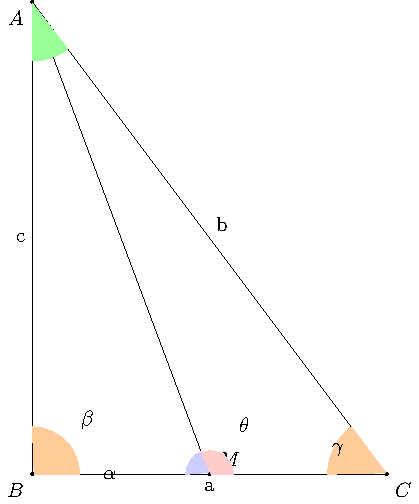
\includegraphics[width=2.0in]{./congurentpicabc.pdf}
				\caption{$\Delta$ ABC}
				\label{fig:triangle}
	    	\end{minipage}
	    	\hfill
	    	\begin{minipage}{0.48\textwidth}
				\centering
				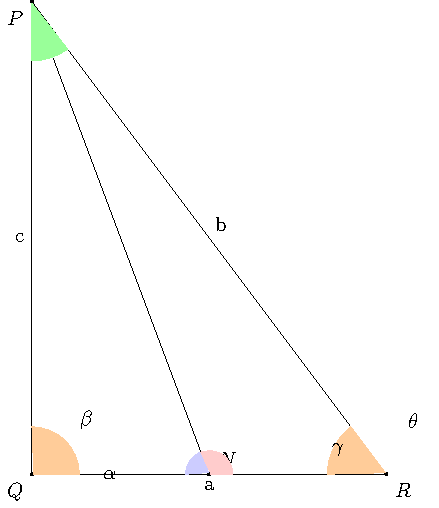
\includegraphics[width=2.0in]{./congurentpicabc2.pdf}
				\caption{$\Delta$ PQR }
				\label{fig:triangle2}
	   	 	\end{minipage}	
    	\end{figure}

		given that $\to$\\
		\begin{align}
			AB = PQ\\
			AM = PN\\
			BC = QR	
		\end{align}
	
		from equation $\left(3\right)$...
	
		\begin{align}
			\frac{BC}{2} = \frac{QR}{2} \\
			BM = QN
		\end{align}

		from fig $\left[1\right]$ and $\left[2\right]$ ...

		\begin{align}
	 		AB = PQ\\
	 		AM = PN\\
	 		BM = QN\\
			\implies  \Delta ABM \cong \Delta PQN
		\end{align}
	
		\item
		given that $\to$\\
		\begin{align}
			AM = PN
		\end{align}
	
		from equation $\left(3\right)$...
	
		\begin{align}
			\frac{BC}{2} = \frac{QR}{2} \\
			MC = NR
		\end{align}
	
	
		from equation $\left(9\right)$...
		\begin{align}
			\Delta ABM \cong \Delta PQN 
			\\
			\implies \angle AMB = \angle PNQ
			\\
			180 - \angle AMB = 180 -  \angle PNQ
			\\
			\angle AMC = \angle PNR
		\end{align}
	
		from equation $\left(10\right)$,$\left(12\right)$ and $\left(16\right)$...
		\begin{align}
			AM = PN
			\\
			MC = NR
			\\
			\angle AMC = \angle PNR
			\\
			\implies  \Delta AMC \cong \Delta PNR
			\\
			\implies AC = PR
		\end{align}
	
		from equation $\left(1\right)$,$\left(3\right)$ and $\left(21\right)$...
		
		\begin{align}
			AB = PQ\\
			BC = QR\\
			AC = QR\\
			\implies  \Delta ABC \cong \Delta PQR
		\end{align}
	
	\end{enumerate}
	
\end{enumerate}


\end{document}